% 
% Annual Cognitive Science Conference
% Sample LaTeX Paper -- Proceedings Format
% 

% Original : Ashwin Ram (ashwin@cc.gatech.edu)       04/01/1994
% Modified : Johanna Moore (jmoore@cs.pitt.edu)      03/17/1995
% Modified : David Noelle (noelle@ucsd.edu)          03/15/1996
% Modified : Pat Langley (langley@cs.stanford.edu)   01/26/1997
% Latex2e corrections by Ramin Charles Nakisa        01/28/1997 
% Modified : Tina Eliassi-Rad (eliassi@cs.wisc.edu)  01/31/1998
% Modified : Trisha Yannuzzi (trisha@ircs.upenn.edu) 12/28/1999 (in process)
% Modified : Mary Ellen Foster (M.E.Foster@ed.ac.uk) 12/11/2000
% Modified : Ken Forbus                              01/23/2004
% Modified : Eli M. Silk (esilk@pitt.edu)            05/24/2005
% Modified : Niels Taatgen (taatgen@cmu.edu)         10/24/2006
% Modified : David Noelle (dnoelle@ucmerced.edu)     11/19/2014
% Modified : Roger Levy (rplevy@mit.edu)     12/31/2018



%% Change "letterpaper" in the following line to "a4paper" if you must.

\documentclass[10pt,letterpaper]{article}

\usepackage{cogsci}

%\cogscifinalcopy % Uncomment this line for the final submission 


\usepackage{pslatex}
\usepackage{apacite}
\usepackage{float} % Roger Levy added this and changed figure/table
                   % placement to [H] for conformity to Word template,
                   % though floating tables and figures to top is
                   % still generally recommended!

%\usepackage[none]{hyphenat} % Sometimes it can be useful to turn off
%hyphenation for purposes such as spell checking of the resulting
%PDF.  Uncomment this block to turn off hyphenation.
\usepackage{graphicx}


%\setlength\titlebox{4.5cm}
% You can expand the titlebox if you need extra space
% to show all the authors. Please do not make the titlebox
% smaller than 4.5cm (the original size).
%%If you do, we reserve the right to require you to change it back in
%%the camera-ready version, which could interfere with the timely
%%appearance of your paper in the Proceedings.

\title{Exploring the contributions of environmental factors in folk categorization}
 
\author{{\large \bf Joshua T. Abbott (joshua.abbott@unimelb.edu.au)} \\
 {\large \bf Charles Kemp (ckemp@unimelb.edu.au)} \\
  School of Psychological Sciences,  \\
  University of Melbourne, 3010, Australia}



\begin{document}

\maketitle


\begin{abstract}
How do we name things? What role does frequency of observation and physical size play in categorization of animals? Here we explore these questions using ideas from anthropology and ethnobiology, and utilizing large-scale citizen science datasets.

\textbf{Keywords:} 
ethnobiology; categorization; bird naming; citizen science
\end{abstract}


\section{Introduction}

What role does frequency of exposure have in being able to determine the name for a bird or its role in a taxonomy? What about the size of the bird? BIG QUESTION: What contributes to naming data?

More generally, we're interested in exploring computational principles that guide the naming and structuring of categories. Following a tradition of ethnobiological classification \cite{berlin1973general,berlin2014ethnobiological}, we aim to explore what kinds of features influence these behaviors. 

These questions are interesting because we typically take for granted the categories of natural kinds. However, scientific taxonomies are just another human-constructed category system. When considering the set of birds in particular, it has been difficult for biologists to agree on a standardized taxonomy, which has been shown to severely impact decisions on conservation policy \cite{peterson2006taxonomy,garnett2017taxonomy}.
% In particular we will explore frequency of observation. (WE'LL WANT SOME COGPSYCH PAPERS ABOUT THIS -- THAT ACTUALLY MIGHT BE A NICE WAY TO FRAME SOME RESULTS LATER -- SHOULD EXPLORE PREVIOUS PAPERS FOR POSSIBLE HYPOTHESES/PREDICTIONS RELATED TO THIS -- e.g., where we use eBird data as the frequency and test predictions against the language data)

What ebird can contribute to the folk biology literature: frequency data.

This connects with the theoretical debate about cognitive vs utilitarian view of classification \cite{hunn1982utilitarian,lopez1997tree}. Frequency data provide some new ways to test the utilitarian view. For example, we could use frequencies to address questions like:

1) do unnamed species tend to have low frequency?

2) if a species is lumped in with another species under the same label -- does one of these species have low frequency?

3) in cases where nomenclature reveals prototype effects -- is the prototype highest in frequency?

For more on point 3 see \cite{berlin1972speculations}:
"A highly regular labeling process can be described for the encoding of
specific taxa, given the primarily binary partition of a generic taxon. In
general, one specific category, because it is most widespread, larger, best
known, or the like, will always be recognized as the typical species of the
folk genus. This taxon can be referred to as the type-specifict, he archetype,
or the ideal type....
As Wyman and Harris have said in referring to Navaho ethnobotany, 'The
situation is as if in our binomial system the generic name were used alone for
the best known species of a genus, while binomial terms were used for all other
 members of the genus'" 



\section{Environmental factors in ethnobiological classification}
Environmental factors have played a major role in scientific classification of species \cite{amadon1943bird}.

Here we talk about the data we use. We show how to utilize publicly available digitized information to explore these questions.

For an official taxonomic system, we follow the Clements taxonomy \cite{clements2007clements}.

\subsection{Language naming data}
We focus on a single language for brevity. We use bird-naming data from \cite{hunn2008zapotec}, also found online\footnote{http://faculty.washington.edu/hunn/zapotec/z5.html}, a Zapotec language spoken in a small village in San Juan Gb\"{e}\"{e}, Oaxaca Mexico.


\subsection{Frequency data}
We utilize a citizen-based bird observation network, eBird \cite{sullivan2009ebird}. We sampled bird observational data from just the region containing the state of Oaxaca, Mexico, for the timespan between Jan 1, 2018 and Jan 1, 2020. This resulted in XXX entries.


\subsection{Physical Size}
Bird weights as an aid in taxonomy \cite{amadon1943bird}.

We'll also look at bird size as a factor, following \cite{hunn1999size} and using data from EltonTraits \cite{wilman2014eltontraits}.  This data set provides information on key attributes for all 9993 and 5400 extant bird and mammal species, derived from key literature sources. Variables include relevance of select diet types and foraging strata, body size, and activity time.

We focus on the body mass data, separately sourced from \cite{dunning2007crc}, which is measured as the geometric mean of average values provided for both sexes.



\section{What categories are given a name?}

\subsection{Frequency}
Here we analyze the frequencies of birds named in Zapotec. We plot the densities of birds named and unamed birds, along with all birds observed in the state of Oaxaca in Figure~\ref{birdfreqviolin}.

\begin{figure}[h!]
	\begin{center}
		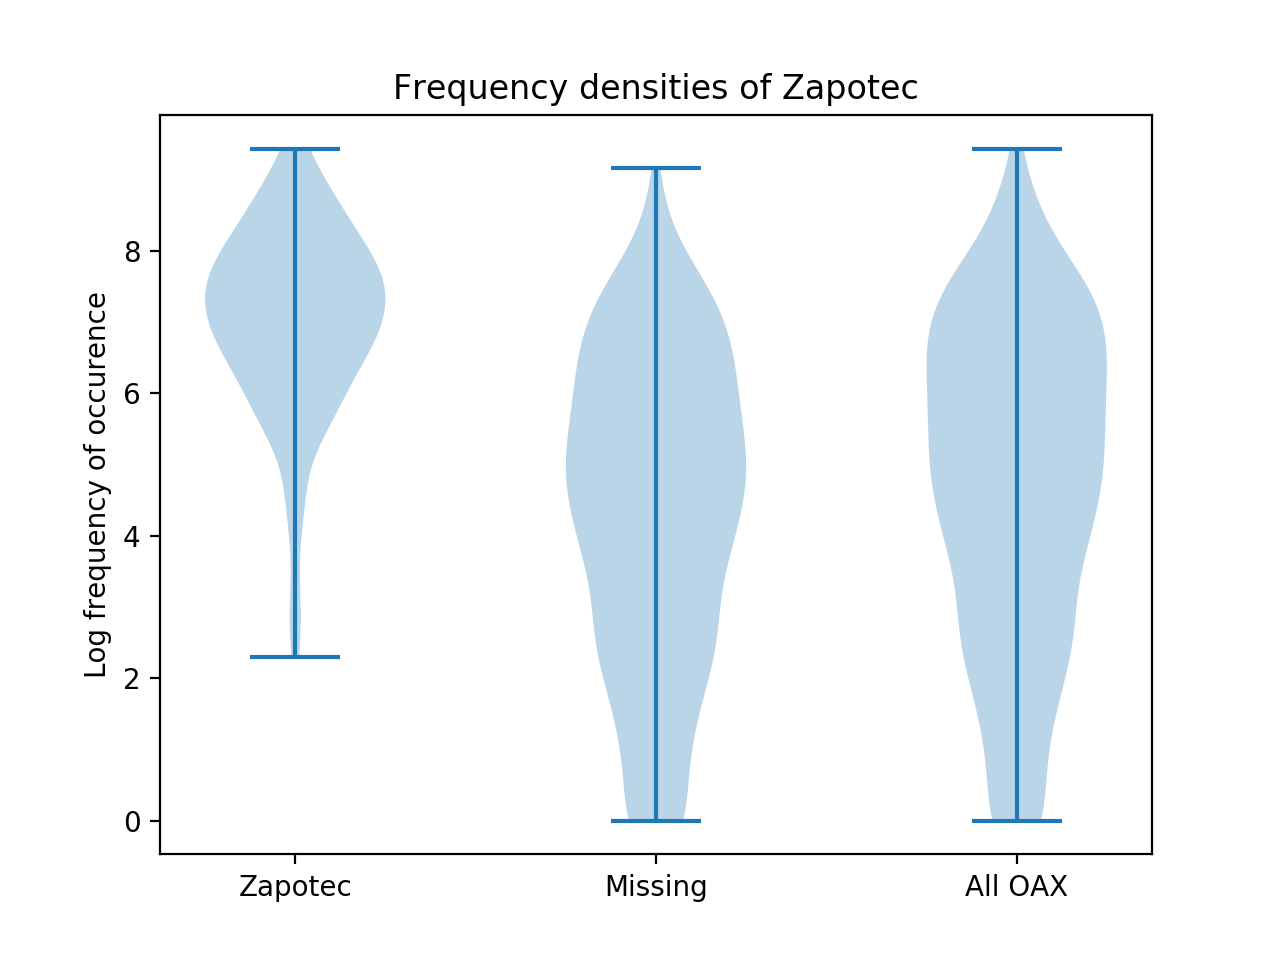
\includegraphics[width=0.5\textwidth]{./figures/birdfreq-violinplots.png}
        \caption{Frequency densities of birds named in Zapotec and those observed in the state of OAX.}
        \label{birdfreqviolin}
	\end{center}
\end{figure}

\subsection{Size}
SSRRs.


\section{Analysis of name-forms}

\subsection{Name-length}
Zipfian?

\subsection{Compound names}
Monomial vs. compound frequencies, sizes?

\subsection{Prototypes}

Here we look at unmarked-prototypes in Hunn's data on Zapotec bird-naming.


\section{Discussion}

This work extends the investigation of language categories using large-scale datasets online \cite{kemp2012kinship,regier2016languages}

\subsection{Future Directions}
The next step would be to expand these analyses to more languages. To do this one needs to find trustworthy ethnographies similar to the Zapotec naming data we used here from \citeA{hunn2008zapotec}, and one needs decent coverage in eBird over the geographic region in question. Clear next steps would be to analyze the Tzeltal language from Chiapas, Mexico, and the Tlingit language from the Pacific Northwest of North America, both published by Hunn as well \cite{hunn1977tzeltal,hunn2012tlingit}, which have decent coverage within their respective geographics regions in eBird observational data. 

That said, it can be difficult to find languages with both expert ethnographries of the folk biological naming systems which also have good coverage in eBird. This has prohibited us from exploring bird naming data from known experts in regions with low coverage in eBird (e.g., naming data summarized in \cite{holman2002relation}, including the Tobelo language from Indonesia \cite{taylor1990folk} and the Anindilyakwa language from Australia \cite{waddy1988classification}, which do not have coverage in eBird currently).

\section{Conclusion}

% \section{Formalities, Footnotes, and Floats}


% The entire content of a paper (including figures, references, and anything else) can be no longer than six pages in the \textbf{initial submission}. In the \textbf{final submission}, the text of the paper, including an author line, must fit on six pages. Up to one additional page can be used for acknowledgements and references.

% The text of the paper should be formatted in two columns with an
% overall width of 7 inches (17.8 cm) and length of 9.25 inches (23.5
% cm), with 0.25 inches between the columns. Leave two line spaces
% between the last author listed and the text of the paper; the text of
% the paper (starting with the abstract) should begin no less than 2.75 inches below the top of the
% page. The left margin should be 0.75 inches and the top margin should
% be 1 inch.  \textbf{The right and bottom margins will depend on
%   whether you use U.S. letter or A4 paper, so you must be sure to
%   measure the width of the printed text.} Use 10~point Times Roman
% with 12~point vertical spacing, unless otherwise specified.

% The title should be in 14~point bold font, centered. The title should
% be formatted with initial caps (the first letter of content words
% capitalized and the rest lower case). In the initial submission, the
% phrase ``Anonymous CogSci submission'' should appear below the title,
% centered, in 11~point bold font.  In the final submission, each
% author's name should appear on a separate line, 11~point bold, and
% centered, with the author's email address in parentheses. Under each
% author's name list the author's affiliation and postal address in
% ordinary 10~point type.

% Indent the first line of each paragraph by 1/8~inch (except for the
% first paragraph of a new section). Do not add extra vertical space
% between paragraphs.


% \section{First Level Headings}

% First level headings should be in 12~point, initial caps, bold and
% centered. Leave one line space above the heading and 1/4~line space
% below the heading.


% \subsection{Second Level Headings}

% Second level headings should be 11~point, initial caps, bold, and
% flush left. Leave one line space above the heading and 1/4~line
% space below the heading.


% \subsubsection{Third Level Headings}

% Third level headings should be 10~point, initial caps, bold, and flush
% left. Leave one line space above the heading, but no space after the
% heading.


% \section{Formalities, Footnotes, and Floats}

% Use standard APA citation format. Citations within the text should
% include the author's last name and year. If the authors' names are
% included in the sentence, place only the year in parentheses, as in
% \citeA{NewellSimon1972a}, but otherwise place the entire reference in
% parentheses with the authors and year separated by a comma
% \cite{NewellSimon1972a}. List multiple references alphabetically and
% separate them by semicolons
% \cite{ChalnickBillman1988a,NewellSimon1972a}. Use the
% ``et~al.'' construction only after listing all the authors to a
% publication in an earlier reference and for citations with four or
% more authors.


% \subsection{Footnotes}

% Indicate footnotes with a number\footnote{Sample of the first
% footnote.} in the text. Place the footnotes in 9~point font at the
% bottom of the column on which they appear. Precede the footnote block
% with a horizontal rule.\footnote{Sample of the second footnote.}


% \subsection{Tables}

% Number tables consecutively. Place the table number and title (in
% 10~point) above the table with one line space above the caption and
% one line space below it, as in Table~\ref{sample-table}. You may float
% tables to the top or bottom of a column, and you may set wide tables across
% both columns.

% \begin{table}[H]
% \begin{center} 
% \caption{Sample table title.} 
% \label{sample-table} 
% \vskip 0.12in
% \begin{tabular}{ll} 
% \hline
% Error type    &  Example \\
% \hline
% Take smaller        &   63 - 44 = 21 \\
% Always borrow~~~~   &   96 - 42 = 34 \\
% 0 - N = N           &   70 - 47 = 37 \\
% 0 - N = 0           &   70 - 47 = 30 \\
% \hline
% \end{tabular} 
% \end{center} 
% \end{table}


% \subsection{Figures}

% All artwork must be very dark for purposes of reproduction and should
% not be hand drawn. Number figures sequentially, placing the figure
% number and caption, in 10~point, after the figure with one line space
% above the caption and one line space below it, as in
% Figure~\ref{sample-figure}. If necessary, leave extra white space at
% the bottom of the page to avoid splitting the figure and figure
% caption. You may float figures to the top or bottom of a column, and
% you may set wide figures across both columns.

% \begin{figure}[H]
% \begin{center}
% \fbox{CoGNiTiVe ScIeNcE}
% \end{center}
% \caption{This is a figure.} 
% \label{sample-figure}
% \end{figure}


% \section{Acknowledgments}

% In the \textbf{initial submission}, please \textbf{do not include
%   acknowledgements}, to preserve anonymity.  In the \textbf{final submission},
% place acknowledgments (including funding information) in a section \textbf{at
% the end of the paper}.


% \section{References Instructions}

% Follow the APA Publication Manual for citation format, both within the
% text and in the reference list, with the following exceptions: (a) do
% not cite the page numbers of any book, including chapters in edited
% volumes; (b) use the same format for unpublished references as for
% published ones. Alphabetize references by the surnames of the authors,
% with single author entries preceding multiple author entries. Order
% references by the same authors by the year of publication, with the
% earliest first.

% Use a first level section heading, ``{\bf References}'', as shown
% below. Use a hanging indent style, with the first line of the
% reference flush against the left margin and subsequent lines indented
% by 1/8~inch. Below are example references for a conference paper, book
% chapter, journal article, dissertation, book, technical report, and
% edited volume, respectively.

% \nocite{ChalnickBillman1988a}
% \nocite{Feigenbaum1963a}
% \nocite{Hill1983a}
% \nocite{OhlssonLangley1985a}
% % \nocite{Lewis1978a}
% \nocite{Matlock2001}
% \nocite{NewellSimon1972a}
% \nocite{ShragerLangley1990a}

\newpage
\bibliographystyle{apacite}

\setlength{\bibleftmargin}{.125in}
\setlength{\bibindent}{-\bibleftmargin}

\bibliography{CogSci2020}


\end{document}
